\chapter{Implementation and results}
\label{kap:kap4}

In this chapter, we describe the implementation of ideas proposed in the previous
chapter and practical results we obtained when measuring experimentally their performance.
This chapter is split into two main parts according to the main topics discussed
in previous chapter namely our new general encoding and decoding routine and hybrid encoding.
In both of these sections, we first describe the important parts and decisions in our
implementation. Subsequently, we describe how we benchmarked our implementation and present
the results we obtained.

The \texttt{C++} source code of our implementation along with all benchmarks can be found
in electronic attachment to this work and also on \texttt{Github}. More about where to
find individual parts of code and how to reproduce our results can be found in appendix A.
All the results presented in this chapter were obtained on a machine with 8-core
AMD~Ryzen~7~2700X with 16~MB of cache, running at 3.7~GHz with 16~GB of RAM. The running
operating system was Ubuntu~20.04.3~LTS. We used both \texttt{GCC} version 9.4.0 and
\texttt{Clang} version 10.0.0 compilers with the optimizations level most of the time
set to \texttt{O3}. Although there are no special hardware requirements, to obtain the
best possible results, our implementation requires a processor with support for \texttt{SSE2}
instruction set.

\section{New decoding method}

\subsection{Implementation}

\paragraph{SDSL library}

We decided to make our solution a part of the \texttt{SDSL} library~\citep{gog2014theory}. This
is one of the most matured and versatile libraries implementing succinct data structures. It is
written in \texttt{C++} and with almost 2\,000 commits from more than 30 contributors, \texttt{SDSL}
is a heavily tested library, offering various implementations of succinct structures such as
wavelet tree, FM-index, bit vector, suffix array and many more. It allows easy use of different
building blocks to implement more complex structures, i.e. using different bit vector implementations
inside of the wavelet tree. On top of this, thorough tests and benchmarks were implemented alongside
the main functionality.

The RRR implementation of bit vector is provided by templated class \texttt{rrr\_vector}
that enables us to use block sizes from 3 up to 256. To support longer block sizes,
\texttt{SDSL} implements 128-bit and 256-bit integers. It generally uses the on-the-fly decoding,
although template specialization for block size 15 that uses the table decoding method is provided.

To support $\access$, \texttt{rrr\_vector} supports single bit access operator \texttt{[]} as well
as \texttt{get\_int} method. To facilitate $\access$ it uses the encoding scheme presented in
Fig.~\ref{obr:RRRFinal} that consists of the array $C$ of fixed size elements that stores classes,
array $O$ of variable length elements that stores offsets of blocks along their class and third array
$P$ that stores pointers to the array $O$, more precisely to the beginning of every superblock.

\texttt{SDSL} uses $\rank$ implementation, where result of $\rank$ is precomputed for the beginning
of every superblock. To answer the query, binary search along the precomputed values is done first.
Then linear search for the final result is made inside of the superblock. As a $\select$ can be answered
using the binary search and $\rank$ functionality, the first part of answering $\select$ is to binary
search between precomputed values of $\rank$, then to do the $\select$ inside of the superblock. This
demonstrates, how the size of superblock can be used to balance the ratio of space used and the speed
of the $\access$, $\rank$ and $\select$ methods. Although size of superblock is one of the parameters
of \texttt{rrr\_vector}, we did not make any changes to the preset number of blocks per superblock that is
set in \texttt{SDSL} to 32.

We decided to use the specialization for block size 15 as an underlying solution for the encoding and
decoding of sub-blocks. We provided specialized implementations for block sizes 31, 63 and 127 that
are mostly used in practical scenarios. We based our implementation on the general implementation of
\texttt{rrr\_vector} and tried to keep the number of changes as small as possible to easily observe the
effects of our new decoding method. We have been able to implement our changes and at the same time alter
only two methods that the \texttt{SDSL} uses for encoding and decoding namely \texttt{bin\_to\_nr(bin)} and
\texttt{nr\_to\_bin(k, nr)}. As we mentioned, the encoding is less performance-critical in most of the
applications as it is done only once when constructing bit vector. This is why we focuse more on the decoding
part of the implementation.

\paragraph{Division of problem into sub-problems}

When implementing our decoding routine, we put most of our focus on the process of dividing problem into
sub-problems of smaller size. This is a part, where we obtain pairs $(c_1, o_1)$ and $(c_2, o_2)$
from the encoded pair $(c, o)$ and call another decoding subroutine on these two pairs.
There are various reasons why we focus on this part of the algorithm. The first one is that for smaller
blocks solving the sub-problems is done using the table approach which is very fast and can be hardly
made faster as it consists only of one table lookup. The second one is that this part is blocking us
from solving the sub-problems and even though sub-problems may be potentially solved somehow in parallel,
e.g. by instruction-level parallelism, this part is harder to parallelize.

Let us now break down the process of dividing the original problem into sub-problems into following 3 steps:
\begin{enumerate}
	\item Finding the class pair $(c_1, c_2)$.
	\item Counting the number of possibilities for first and second sub-block $\text{comb}_1, \text{comb}_2$.
	\item Compute offsets of sub-blocks $o_1$ and $o_2$.
\end{enumerate}
The most trivial part is third step as it only consists of a number of arithmetic operations. Then,
second step, that is a computation of $\text{comb}_1$ and $\text{comb}_2$. We know that $\text{comb}_1$
and $\text{comb}_2$ is equal to ${b\choose c_1}$ and ${b\choose c_2}$, respectively. These two numbers
can be computed beforehand as there are only roughly $b^2$ combinations of possible pairs of $c$ and $c_1$.
So roughly at the price of two cache misses, we can easily do the last two steps. To solve the first step,
we may precompute for every possible class $c$, numbers $C_0, C_1,\ldots ,C_{c}$ where $C_i$ is the number
of blocks along the class $c$ with their class pair equal to $(i, c-i)$. Example can be observed in
Fig.~\ref{table:class_pairs}.

\begin{figure}
	\centerline{
        \begin{tabular}{c c c c}
            $C_k$	&	$(c_1, c_2)$  &   Block count & Offsets of blocks\\
        \hline
			$C_0$	&	$(0, 2)$	&   \tt 3 	&	0-2\\
			$C_1$	&	$(1, 1)$	&	\tt 9 	&	3-11\\
			$C_2$	&	$(2, 0)$	&	\tt 3	&	12-14\\
        \end{tabular}
	}
	\caption[TODO]{
        The table shows all the class pairs with the number of blocks for $b=6, c=2$.
    }
	\label{table:class_pairs}
\end{figure}

We would like to map the offset of the block to the number $C_i$ and thus identify $i$,
the number of ones in the first and thus also second sub-block. One possible way how to
do this is to precompute the prefix sums over these numbers such that $$P_i = \sum_{j=0}^{i} C_i.$$
As these prefix sums form an increasing sequence, we can binary search for class that contains our offset.

Although binary search has good time complexity, the number of buckets where our offset
may land is usually small. As we found out, linear search outperforms binary search most
of the time. Another idea that we tested was to speed up the linear search using the
\texttt{SIMD} instructions. These can be used to do 4 comparisons at a time using special
128-bit register. In practice, we found that sequential search using the \texttt{SIMD}
instructions leads to the best results for smaller block sizes. Possible implementations
that we tested, follow in listings \ref{code:linear}, \ref{code:linearSimd} and \ref{code:binary}.
The naming convention adheres to \texttt{SDSL} naming of $k$ for class, $nr$ for offset.
To simplify naming, if block $B$ was encoded using division to sub-blocks $B_1$ and
$B_2$ such that $B=B_1\cdot B_2$ then we call the $B_1$ the \textit{left sub-block} and
consequently its class $\text{left\_k}$ while $B_2$ is called \textit{right sub-block}.

\lstset{language=C++,caption={Linear search for classes of sub-blocks},label=code:linear}
\begin{lstlisting}
uint32_t get_left_class(uint8_t k, uint32_t nr)  {
	int left_k_from = std::max(k - 15, 0);
	int left_k_to = std::min(k, 15);
	int left_k = left_k_from;
	for (; left_k < left_k_to; ++left_k)  {
		uint32_t curr_index = P[k][left_k+1];
		if (curr_index >= nr)  {
			if (curr_index == nr)
				++left_k;
			break;
		}
	}
	return left_k;
}
\end{lstlisting}

\lstset{language=C++,caption={SIMD enhanced linear search for classes of sub-blocks},label=code:linearSimd}
\begin{lstlisting}
uint32_t get_left_class(uint8_t k, uint32_t nr)  {
	int left_k_from = std::max(k - 15, 0);
	int left_k_to = std::min(k, 15);
	__m128i keys = _mm_set1_epi32(nr);
	__m128i vec1 =
		_mm_loadu_si128(reinterpret_cast<__m128i*>(&P[k][0]));
	__m128i vec2 =
		_mm_loadu_si128(reinterpret_cast<__m128i*>(&P[k][4]));
	__m128i vec3 =
		_mm_loadu_si128(reinterpret_cast<__m128i*>(&P[k][8]));
	__m128i vec4 =
		_mm_loadu_si128(reinterpret_cast<__m128i*>(&P[k][12]));

	__m128i cmp1 = _mm_cmpgt_epi32(vec1, keys);
	__m128i cmp2 = _mm_cmpgt_epi32(vec2, keys);
	__m128i cmp3 = _mm_cmpgt_epi32(vec3, keys);
	__m128i cmp4 = _mm_cmpgt_epi32(vec4, keys);

	__m128i tmp1 = _mm_packs_epi32(cmp1, cmp2);
	__m128i tmp2 = _mm_packs_epi32(cmp3, cmp4);
	uint32_t mask1 = _mm_movemask_epi8(tmp1);
	uint32_t mask2 = _mm_movemask_epi8(tmp2);

	uint32_t mask = (mask2 << 16) | mask1;

	int left_k = left_k_to;

	if (mask != 0)
	{
		left_k = (1 + __builtin_ctz(mask)) / 2;

		if (P[k][left_k] > nr)
			--left_k;
	}
	return left_k;
}
\end{lstlisting}

\lstset{language=C++,caption={Binary search for classes of sub-blocks},label=code:binary}
\begin{lstlisting}
uint32_t get_left_class(uint8_t k, uint32_t nr)  {
	int left_k_from = std::max(k - 15, 0);
	int left_k_to = std::min(k, 15);
	auto it = std::upper_bound(P[k].begin() + left_k_from,
                                     P[k].begin() + left_k_to, nr);
    int left_k = std::distance(P[k].begin(), it);
    if (P[k][left_k] > nr)
      --left_k;
	return left_k;
}
\end{lstlisting}

\paragraph{Choosing the right sub-problem size}

In previous chapter, we showed that our method can take encoding and decoding subroutines
of sizes $b_1$ and $b_2$ and combine them together to obtain routine for encoding and
decoding of size $b_1+b_2$. Thus it is up to us, how we obtain the decoding for block sizes
bigger than 15. Minor inconvenience is, that the most used block sizes are of form $2^i-1$.
Combining two block sizes of this form, however, leads only to block size of length $2^j-2$
so to obtain the usable block length, we need to "extend" this solution by one bit.

As we wanted to base our solutions on table decoding routine for block size 15, it is most
reasonable to obtain the next interesting block size - 31, by at first splitting block into
single-bit and 30-bit sub-problem and then obtaining 30-bit solution using two 15-bit
subroutine calls. For 63, the next interesting block size, there are unfortunately more
possible combinations that make sense. We may combine solution for single-bit and 62-bits
and then obtain 62-bit block size using combination of solution for block size 31. On the
other hand, it may be more beneficial, to do 63-bit block size by splitting it into 3 bits
and 60 bits. Thus, before choosing what solution we want to fully include into \texttt{SDSL},
we explored and tried several promising combinations and microbenchmarked them.

\subsection{Experimental results}

We benchmarked our code using two types of benchmarks. The first type of benchmarks
used a \texttt{Google Benchmark} library. This is one of the standard libraries used to
microbenchmark code. A code snippet that is being benchmarked is run several times until
stable results are obtained. This makes the results reliable even if the measured time is
very small and also limits the interference of other running processes on the result of
benchmark. Although reliable, this types of benchmarks are more artificial in nature and
do not give a best sense, how the solution may behave on real data. The second type of
benchmarks used were the ones that are included in \texttt{SDSL}. These are built on top
of a data from the \texttt{Pizza\&Chili} datasets \citep{ferragina2005pizza} and include
many types of data such as DNA sequences, \texttt{C} and \texttt{Java} source codes from
\texttt{Linux} and \texttt{GCC} projects as well as English texts from the Gutenberg project.
More information about this data such as some statistics about the compressibility and much
more can be found in section 4.2 of \cite{ferragina2009compressed}. We only provide information
necessary to explain the measured phenomenons later when exploring the results of our benchmarks. 

\paragraph{Microbenchmarks of block decoding}

\begin{figure}
	\centerline{
	\begin{tabular}{|l|l|r|}
		\hline
		Block size &	Method									&	$\mu s$ per 1k queries \\
		\hline
		\multirow{2}{*}{15} & SDSL\_Table                         	&    2  \\
							& SDSL\_ON\_THE\_FLY  					&   45  \\
		\hline
		\multirow{4}{*}{30} & OUR\_LINEAR\_15\_15                 	&   9  \\
							& OUR\_SIMD\_15\_15                   	&   8  \\
							& OUR\_BINARY\_15\_15                 	&  15  \\
							& SDSL\_ON\_THE\_FLY  					&  93  \\
		\hline
		\multirow{2}{*}{31} & OUR\_LINEAR\_1\_30                  	&  11  \\
							& SDSL\_ON\_THE\_FLY  					&  96  \\
		\hline
		\multirow{3}{*}{62} & OUR\_LINEAR\_31\_31                 	&  36  \\
							& OUR\_BINARY\_31\_31                 	&  42  \\
							& SDSL\_ON\_THE\_FLY  					& 130  \\
		\hline
		\multirow{3}{*}{63} & OUR\_LINEAR\_1\_62                  	&  33  \\
							& OUR\_LINEAR\_3\_30\_30              	&  32  \\
							& SDSL\_ON\_THE\_FLY  					& 148  \\
		\hline
		\multirow{2}{*}{127} & OUR\_LINEAR\_1\_63\_63             	&  88  \\
							 & OUR\_BINARY\_1\_63\_63             	&  91  \\
		\hline
	\end{tabular}
	}
	\caption[TODO]{Results of microbenchmarking various types of decoding implementations.
	The numbers in method name denote to what block sizes the problem was broken. The name
	reflects what method was used to broke the problem into subproblems.
	}
	\label{obr:simple_benchmark}
\end{figure}

These benchmarks were used in the early stage of the development to measure a potential gain from
our new method of encoding and decoding. We mainly focused on measuring different block sizes
in combination with different methods used for dividing block to subproblems and with different
approaches to obtain particular block size. The mainly tested block sizes were 15, 30, 31, 62, 63
and 127. Sizes 15, 31, 63 and 127 are most useful in practice however they can be obtained using
different combinations of block size 30 and 62, i.e. 31 can be combined as 1 bit and 30 bit solution,
63 can be divided to 1 and 62 as well as to 3 and two sub-problems of length 30. Although, these
tests are not made on real life data, they were mainly used as an indication which implementations
are interesting and should be the best candidates for further evaluation.

We used 3 different techniques to divide a problem into sub-problems, these were the linear scan,
binary search and linear scan enhanced by \texttt{SIMD} instructions. In order to implement the
solution for 127 bit block size, we used the 128 bit type \texttt{\_\_uint128\_t} provided by both
\texttt{GCC} and \texttt{Clang} compilers. This type is implemented on platform \texttt{x86\_64}
as a combination of two 64 bit numbers. We compared these results with the table decoding specialization
in \texttt{SDSL} and with on-the-fly decoding for all the other block sizes. The data we run the decoding
on were radomly generated. To generate them, we picked 1\,000 pairs of class and offset by first randomly
picking class of the block and then the offset along this class. The results we measured are shown in
Fig.~\ref{obr:simple_benchmark}.

\paragraph{Bit vector on real data}

After bencharking and finding the potential for speeding up the bit vector implementation using
our new method, we decided to implement and test it in environment that is closer to the real-life
usage of bit vectors. We picked a benchmarking part of \texttt{SDSL} library that tests bit vector
on a randomly generated sequence with fixed number of ones and on raw representation of a wavelet
tree built on top of data from the DNA sequence, XML web data taken from \texttt{DBLP}, computer
science bibliography. Among the explored dimensions is block size and size of the underlying data.
\texttt{SDSL} generates $\access$, $\rank$ and $\select$ queries randomly. We were not able
to find significant practical usability for other access patterns and thus stick with this one.
As a baseline, we choose the 15 bit specialized implementation already implemented in \texttt{SDSL}
that uses the table decoding method. We present the measured results of our and the original
implementation in Fig.~\ref{obr:benchmark_sdsl_new_method}.
\begin{figure}
	\centerline{
		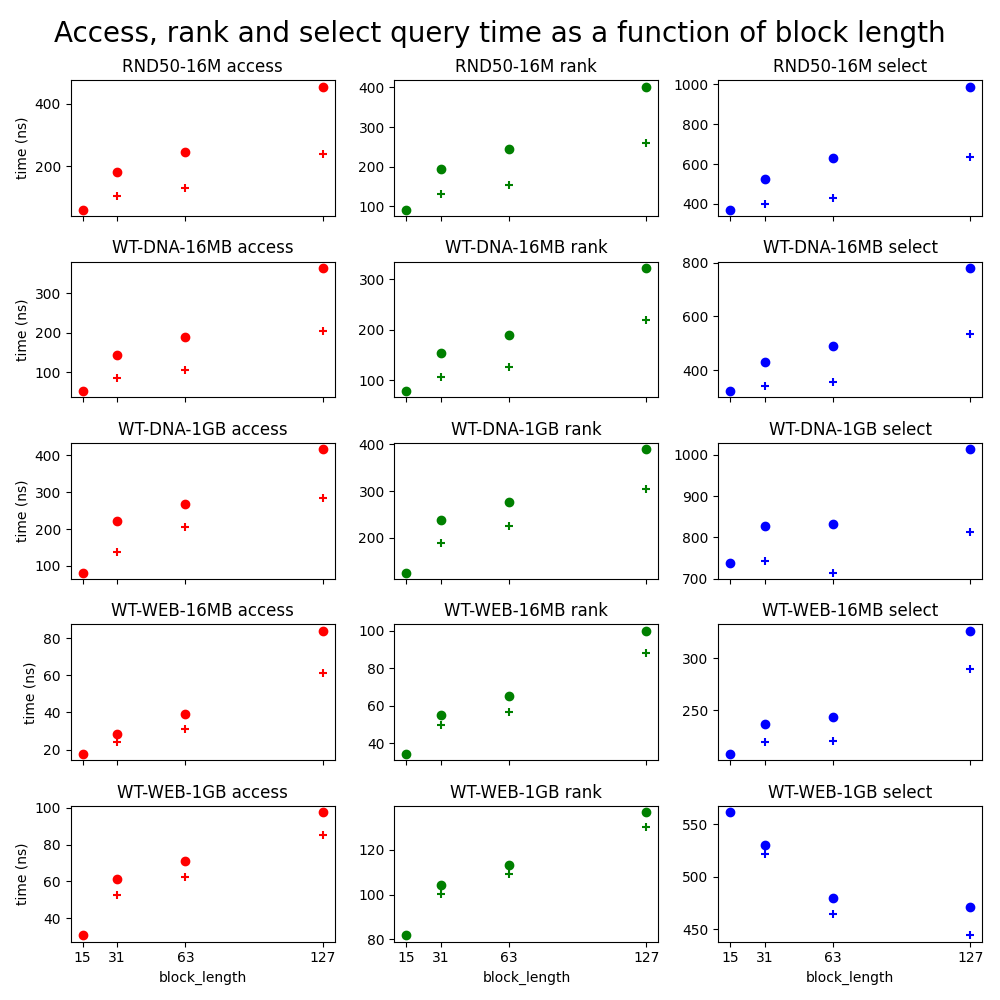
\includegraphics[width=\textwidth, height=0.7\textheight]{images/benchmark_sdsl_new_method}
	}
	\caption[TODO]{\texttt{SDSL} benchmark to measure the bit vector performance and its dependence
	on the block size. Our implementations are marked using cross.
	}
	\label{obr:benchmark_sdsl_new_method}
\end{figure}

There are several interesting things to observe in these results. We can see that our new implementation
beats older implementations on almost all block sizes and all types of data. Note, that results are more
clear on random data and DNA data. On web data, however, the difference is less noticable. We attribute
this behaviour to the fact, that was observed by \cite{gog2014optimized}, creators of this dataset. They
observed that the number of uniform blocks (full of either zeroes or ones) is much bigger in \texttt{WT-WEB}
data than in \texttt{WT-DNA}. For block size 63, they observed ratio of uniform blocks in \texttt{WT-WEB-1GB}
to be 84\% compared to 28\% in \texttt{WT-DNA}. As the uniform blocks are decoded trivially in both
implementations, this makes less opportunities for our implementation to save time. Another visible pattern
is that with increasing block size, the query time generally goes up as decoding takes more and more time.
On the other hand, on query $\select$ in \texttt{WT-WEB} data we can observe, that at the beginning the query
time decreases with increasing block size. This is because time savings of binary search in precomputed $\rank$
values offset growing decoding time.

\paragraph{Bit vector in FM-index}

Even if previous benchmark was done on real data, it was not done in application that is
practically useful. Thus, we further benchmarked our bit vector implementation as a part
of Huffman shaped wavelet tree used inside of the FM-index. Implementation of FM-index in
\texttt{SDSL}, as most of other implementations of FM-index, provides mainly 3 methods:
\begin{itemize}
	\item $\countOp(P)$ - returns the number of occurrences of $P$ in text $T$
	\item $\locateOp(P)$ - returns all positions of pattern $P$ in text $T$
	\item $\extractOp(i, j)$ - returns the subsequence $T[i..j]$
\end{itemize}
The reason that the $\extractOp$ method is useful and non-trivial is that FM-index
does not store the original sequence $T$ -- at least not in an easily readable form.

These benchmarks are provided by $\texttt{SDSL}$ library. They are based on data from
the \texttt{Pizza\&Chili} dataset and use mainly methodology proposed by \cite{ferragina2009compressed}.
The data we used are English texts from Gutenber project, source codes, DNA and protein
sequences. In most of these benchmarks, we used as a baseline the FM-index version based
on uncompressed bit vector. For informative purposes, we also included the version based
on block size 15, using the table decoding, and sparse bit vector.

To benchmark operation $\countOp$, the index over the text is built. Then, random patterns of
various lengths are extracted from the text and subsequently used for benchmarking. Code
that generates these patterns in \texttt{SDSL} is a slight modification of a version provided
by \texttt{Pizza\&Chili}. We measure, as in other places where this benchmark was used, the
ratio between space used for index and the speed normalized by the number of symbols contained
in all searched patterns. We present the results in Fig.~\ref{obr:benchmark_sdsl_count}.

\begin{figure}
	\centerline{
		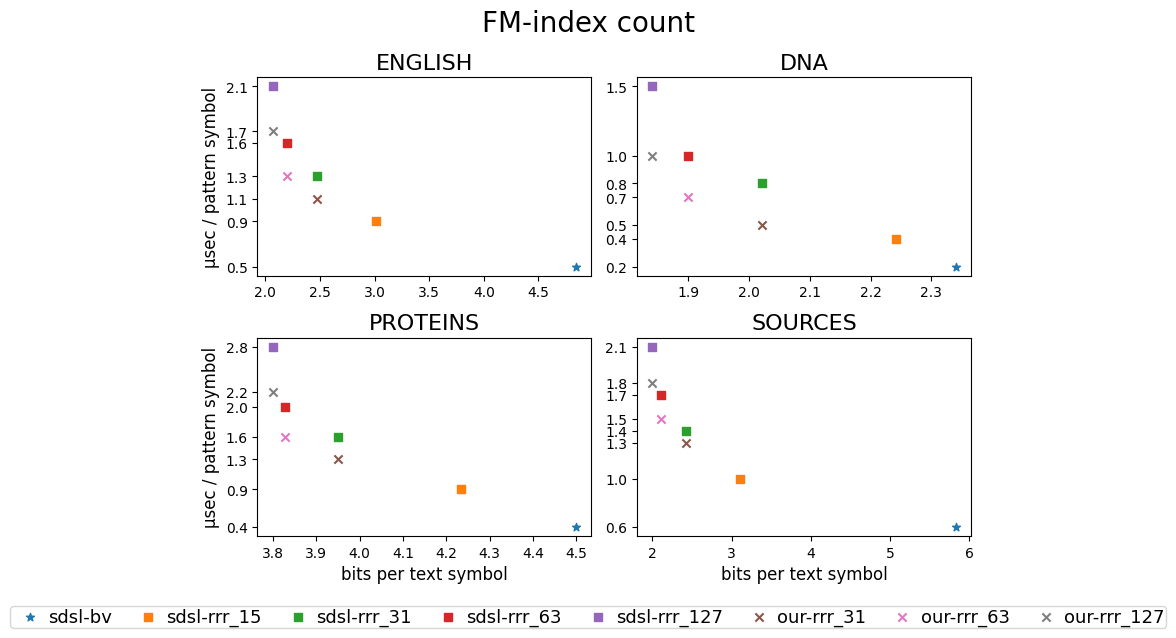
\includegraphics[width=\textwidth, height=0.4\textheight]{images/vysledky_sdsl_count}
	}
	\caption[TODO]{Counting occurences of patterns in various different texts. Displaying
	the query time per pattern symbol for various block sizes and the size of index over the
	text. Uncompresed bit vector and sparse array are included for reference. 
	}
	\label{obr:benchmark_sdsl_count}
\end{figure}

For benchmarking of operation $\extractOp$, \texttt{SDSL} uses a methodology proposed by
\cite{ferragina2009compressed} in Section~5.4. This consists of extracting numerous
substrings of length 512 starting at random positions in text. The additional parameter
that is explored in this benchmark is sampling rate of suffix array and inverse suffix array.
This is basically a parameter that can be used to balance between the speed of FM-index and
its memory usage. Options for this sampling ratio are by default the powers of 2 from 4 up to
256. We show the results for sampling rate equal to 16 in Fig.~\ref{obr:benchmark_sdsl_extract}.
Note that the trends that can be seen in these results are the same for every sampling rate.

\begin{figure}
	\centerline{
		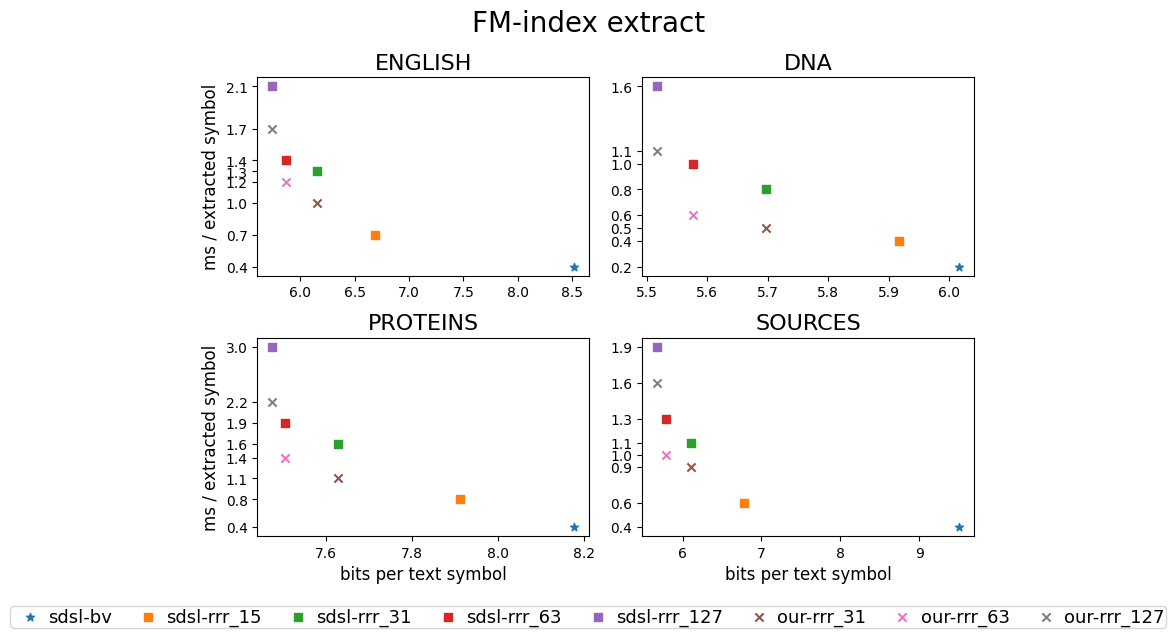
\includegraphics[width=\textwidth, height=0.4\textheight]{images/vysledky_sdsl_extract}
	}
	\caption[TODO]{Extracting parts of the represented text. Displaying
	the query time per extracted symbol for various block sizes and the size of index over the
	text. Uncompresed bit vector and sparse array are included for reference. 
	}
	\label{obr:benchmark_sdsl_extract}
\end{figure}

Benchmarking of operation $\locateOp$ again uses a methodology proposed by \cite{ferragina2009compressed} 
in Section~5.3. This consists of at first locating random patterns of length 5 in the text such
that 2--3 millions of occurences are found in the text. We present our results in Fig.~\ref{obr:benchmark_sdsl_locate}.

\begin{figure}
	\centerline{
		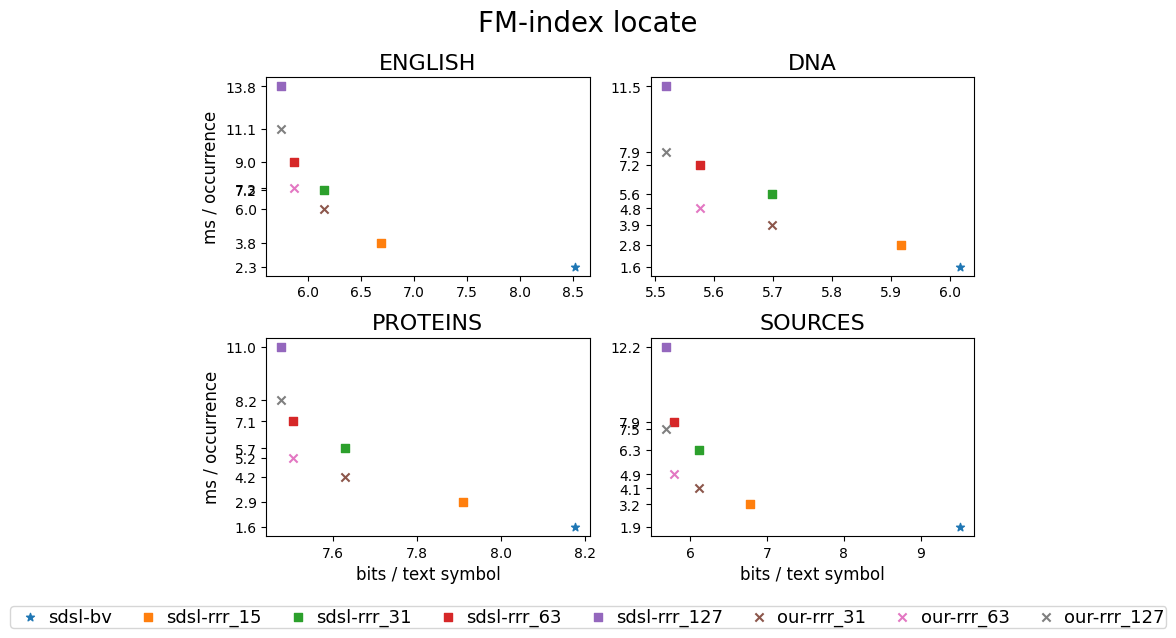
\includegraphics[width=\textwidth, height=0.4\textheight]{images/vysledky_sdsl_locate}
	}
	\caption[TODO]{Locating occurences of patterns in the represented text. Displaying
	the query time per occurence for various block sizes and the size of index over the
	text.
	}
	\label{obr:benchmark_sdsl_locate}
\end{figure}

\paragraph{Correctness}

On top of making sure that our solution is as fast possible we also wanted to make sure it is
correct. We used mainly two types of tests for this purpose. The first are the tests of $\access$,
$\rank$ and $\select$ functionality in \texttt{SDSL} that run mainly on smaller bit sequences
but cover special cases such as bit vector full of zeroes/ones and certain special patterns
that are not encountered often in practice. The second type of tests used was the benchmark
running on wavelet tree representation of real data. Alongside the individual timings, this
benchmark produces, as a checksum, sum of all the results of the $\access$, $\rank$ and $\select$
queries. These checksums can be compared between our and original implementation.

\section{Hybrid encoding}

\subsection{Implementation}

Implementing hybrid encoding required changes to more than encoding and decoding
subroutines. The first necessary change is addition of hybrid cutoff parameter
to the \texttt{rrr\_vector} class and reimplementation of function \texttt{space\_for\_bt(c)}
that is used in \texttt{SDSL} to get the number of bits that are needed to store offset
of block with class $c$. The second change, more impactful on a runtime
of \texttt{rrr\_vector}, relates to the way how we work with superblocks.

When computing $\rank$ of a bit in particular block, we can still binary search for
the superblock where the $i$-th one is located. Then, to linearly search for a result
inside of the superblock, we needed only information from the array of classes $C$.
This is because this array stores the number of ones in the blocks and we can linearly
search for the answer using successive entries of $C$. When we overrun the block, where
the result is located, we go back and find finally answer to $\rank$ inside of a single
block. To locate the beginning of this smaller block, we take the offset of the superblock
in $O$ and add the offset of this block from the beginning of superblock that can be
counted along with the linear search for $\rank$ result. With cutoff in place, however,
we are not able to linearly scan through the superblock only using information contained
in $C$. This is because now, for some classes, $C$ does not store the number of ones in
the block. Thus when we are linearly searching for the result of $\rank$ query along the
block, we need to also from time to time count number of ones for some block in $O$. This
creates some additional memory accesses that may slow down the hybrid implementation.

\lstset{language=C++,caption={Rank query, SDSL implementation (pseudo-code)},label=code:binary}
\begin{lstlisting}
int rank(int i)
{
	int block_idx = i/BLOCK_SIZE;
	int superblock_index = block_idx/BLOCKS_PER_SUPERBLOCK;
	int offset = P[superblock_idx];
	int rank  = R[superblock_idx]; // precomputed rank for superblock
	for (int j = superblock_idx*BLOCKS_PER_SUPERBLOCK; j < block_idx; ++j) {
		uint16_t r = C[j];
		rank  += r;
		offset += rrr_helper::space_for_class(r);
	}
	uint16_t off = i % BLOCK_SIZE;
	if (!off) {
		return rank;
	}
	uint16_t c = C[block_idx];

	uint16_t block_length = rrr_helper::space_for_class(c);
	uint32_t o = rrr_helper::get_blocks_offset(O, offset, block_length);
	uint16_t popcnt  = __popcount(rrr_helper::nr_to_bin(c, o) << (32-off));
	return rank + popcnt;
}
\end{lstlisting}

\lstset{language=C++,caption={Rank query, hybrid implementation (pseudo-code)},label=code:binary}
\begin{lstlisting}
int rank(int i)
{
	int block_idx = i/BLOCK_SIZE;
	int superblock_index = block_idx/BLOCKS_PER_SUPERBLOCK;
	int offset = P[superblock_idx];
	int rank  = R[superblock_idx]; // precomputed rank for superblock
	for (int j = superblock_idx*BLOCKS_PER_SUPERBLOCK; j < block_idx; ++j) {
		uint16_t r = C[j];
		if (r >= c_k) {
			uint32_t o = rrr_helper::get_blocks_offset(O, offset, BLOCK_SIZE);
			rank += __popcount(btnr);
		}
		else {
			rank  += r;
		}
		offset += rrr_helper::space_for_class(r);
	}
	uint16_t off = i % BLOCK_SIZE;
	if (!off) {
		return rank;
	}
	uint16_t c = C[block_idx];

	uint16_t block_length = rrr_helper::space_for_class(c);
	uint32_t o = rrr_helper::get_blocks_offset(O, offset, block_length);
	uint16_t popcnt  = __popcount(rrr_helper::nr_to_bin(c, o) << (32-off));
	return rank + popcnt;
}
\end{lstlisting}

\paragraph{Hybrid version for balanced sequences}

Before implementing our second version of hybrid encoding, we have been interested in a potential
space saving on some real-life data so we analyzed what is the space saved when using hybrid encoding
on a data \texttt{WT-WEB-1GB} and \texttt{WT-DNA-1GB}. The results in Fig.~\ref{obr:hybrid_space_saved}
show, that there is a potential to save some space for certain cutoff values.

\begin{figure}
	\centerline{
	\begin{tabular}{|l|l|r|}
		\multicolumn{3}{c}{WT-DNA-1GB} \\
		\hline
		Block size 			& $c_k$					&  space used by hybrid \\
		\hline
		\multirow{2}{*}{31} & 7                  	&  90\%  \\
							& 15  					&  97\%  \\
		\hline
		\multirow{3}{*}{63} & 7                 	&  93\%  \\
							& 15                 	&  97\%  \\
							& 31  					&  100\%  \\
		\hline
		\multirow{4}{*}{127}& 7                 	&  99\%  \\
							& 15                 	&  99\%  \\
							& 31  					&  101\%  \\
							& 63  					&  102\%  \\
		\hline
	\end{tabular}
	\hspace{3em}
	\begin{tabular}{|l|l|r|}
		\multicolumn{3}{c}{WT-WEB-1GB} \\
		\hline
		Block size 			& $c_k$					&  space used by hybrid \\
		\hline
		\multirow{2}{*}{31} & 7                  	&  73\%  \\
							& 15  					&  85\%  \\
		\hline
		\multirow{3}{*}{63} & 7                 	&  78\%  \\
							& 15                 	&  84\%  \\
							& 31  					&  91\%  \\
		\hline
		\multirow{4}{*}{127}& 7                 	&  94\%  \\
							& 15                 	&  94\%  \\
							& 31  					&  94\%  \\
							& 63  					&  95\%  \\
		\hline
	\end{tabular}
	}
	\caption[TODO]{TODO.
	}
	\label{obr:hybrid_space_saved}
\end{figure}

The major difference from the previous version of hybrid encoding are two helper
functions that are used for mapping or as we call it compressing and decompressing
the blocks class before any of its use.

\lstset{language=C++,caption={Compressing blocks class},label=code:hybrid_valley_compress}
\begin{lstlisting}
int compress_class(int k) {
	if (!is_hybrid_impl) return k;
	if (k < cut_from) {
		return k;
	}
	else if (k <= cut_to) {
		return cutoff;
	}
	else {
		return k-(cut_to-cut_from+1);
	}
}
\end{lstlisting}

\lstset{language=C++,caption={Decompressing blocks class},label=code:hybrid_valley_decompress}
\begin{lstlisting}
int decompress_class(int k) {
	if (!is_hybrid_impl) return k;
	if (k < cut_from) {
		return k;
	}
	else if (k == cutoff) {
		return cut_to;
	}
	else {
		return k+(cut_to-cut_from+1);
	}
}
\end{lstlisting}

\subsection{Experimental results}

\begin{figure}
	\centerline{
		\includegraphics[width=\textwidth, height=0.4\textheight]{images/benchmark_sdsl_hybrid}
	}
	\caption[TODO]{\texttt{SDSL} benchmark to measure the bit vector performance and its dependence
	on the block size. Our implementations are marked using cross.
	}
	\label{obr:benchmark_sdsl_hybrid}
\end{figure}

\begin{figure}
	\centerline{
		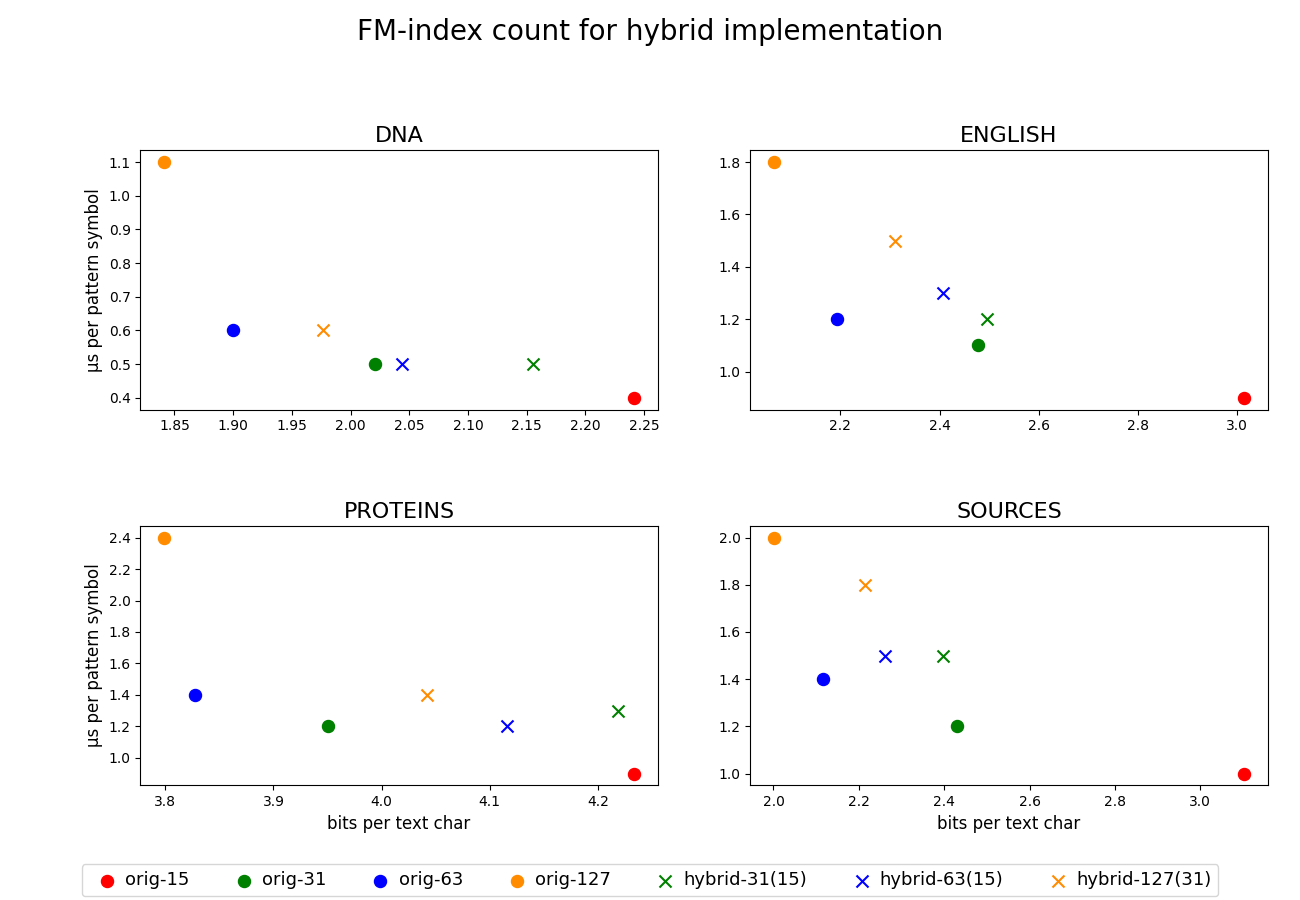
\includegraphics[width=\textwidth, height=0.4\textheight]{images/vysledky_sdsl_hybrid_count}
	}
	\caption[TODO]{TODO: Zatial iba placeholder obrazok.
	}
	\label{obr:benchmark_sdsl_hybrid_count}
\end{figure}

%\begin{figure}
%	\centerline{
%		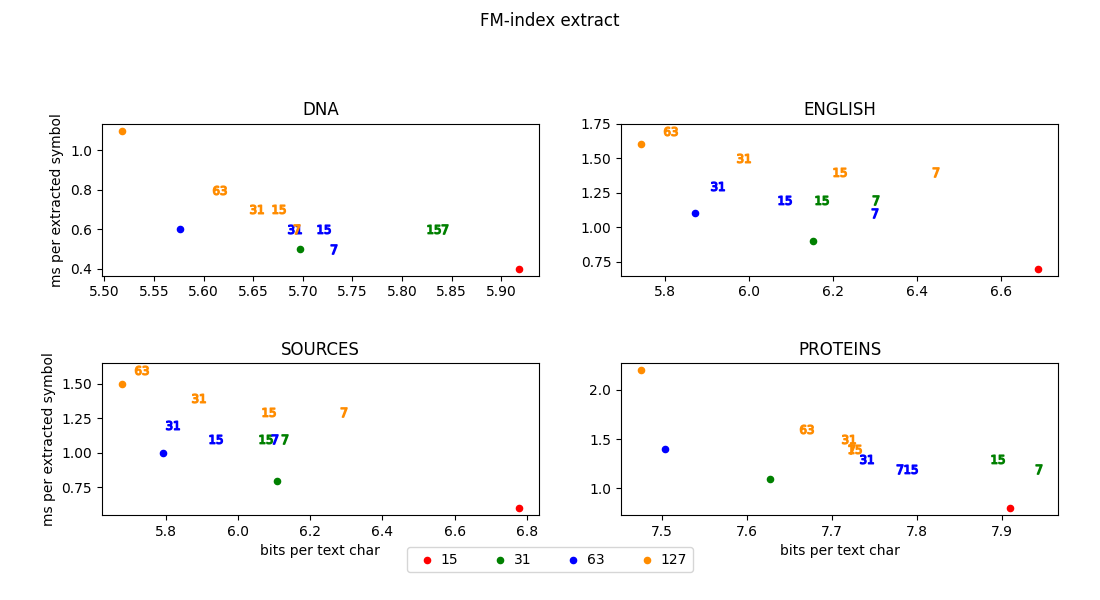
\includegraphics[width=\textwidth, height=0.4\textheight]{images/vysledky_sdsl_hybrid_extract}
%	}
%	\caption[TODO]{TODO
%	}
%	\label{obr:benchmark_sdsl_hybrid_extract}
%\end{figure}

% TODO: FM-indexove grafy